% Created 2021-01-07 Thu 13:59
% Intended LaTeX compiler: pdflatex
\documentclass[presentation]{beamer}
\usepackage[utf8]{inputenc}
\usepackage[T1]{fontenc}
\usepackage{graphicx}
\usepackage{grffile}
\usepackage{longtable}
\usepackage{wrapfig}
\usepackage{rotating}
\usepackage[normalem]{ulem}
\usepackage{amsmath}
\usepackage{textcomp}
\usepackage{amssymb}
\usepackage{capt-of}
\usepackage{hyperref}
\usetheme{Boadilla}
\author{Abraham Raji}
\date{October 2, 2020}
\title{Sustainable Digital Agriculture}
\titlegraphic{
\includegraphics[height=.1\textheight]{./images/logo.jpeg}}
\subtitle{with the help of Robotics,IoT and Open Data}}
\institute[EI, SJCET]{Guide: Ms. Rashmi Annamma George}
\hypersetup{
 pdfauthor={Abraham Raji},
 pdftitle={Sustainable Digital Agriculture},
 pdfkeywords={iot agriculture},
 pdfsubject={with the help of Robotics,IoT and Open Data},
 pdfcreator={Emacs 27.1 (Org mode 9.5)}, 
 pdflang={English}}
\begin{document}

\maketitle

\section*{Introduction}
\label{sec:orgf94668c}
\begin{frame}[label={sec:org66d0e8c}]{Agriculture in the Indian context}
\begin{itemize}
\item Three fourths of the India population workforce is related with
\end{itemize}
agriculture and its allied fields.
\begin{itemize}
\item Most farmers in the country still practice traditional methods
\end{itemize}
for agriculture.
\begin{itemize}
\item These practices have not yet been attuned to the recent
\end{itemize}
climate change phenomenon.
\begin{itemize}
\item As a result the gross yield produced is getting reduced year
\end{itemize}
after year.
\end{frame}
\begin{frame}[label={sec:org87719b3}]{Paddy Cultivation Kerala}
\begin{figure}[htbp]
\centering
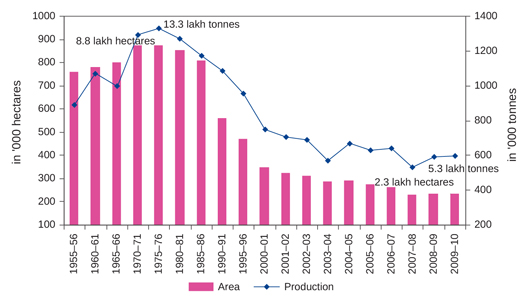
\includegraphics[width=.9\linewidth]{./images/graph.png}
\caption{Paddy Cultivation in Kerala, Jayan Jose Thomas, Department of Humanities and Social Sciences, Indian Institute of Technology, New Delhi}
\end{figure}
\end{frame}
\begin{frame}[label={sec:org6f1bcee}]{Difficulties faced by farmers}
\begin{itemize}
\item The agriculture concern on three major areas that is inadequate water
supply (irrigation), attack of crops by pests and insects and thirdly failure
in properly storing the produce which in turn might be attacked by pests and
rodent. \footnote{Sudhir Rao Rupanagudi, Ranjani B. S., Prathik Nagaraj, Varsha G Bhat,
and Thippeswamy G, A Novel Cloud Computing based Smart Farming System
for Early Detection of Borer Insects in Tomatoes, ICCICT, pp.1-6, 2015.}
\item We have reached a point in human history where we are able
to carry computers in our pockets and have expored
possibilities we've nerver been able to do so before. It is about
time that we now implement out technological prowess as a
race to improve basic necessities such as food.
\end{itemize}
\end{frame}
\begin{frame}[label={sec:orgec7c3e9}]{Difficulties faced by farmers}
\begin{itemize}
\item The concept of IOT can be used in agriculture field. In this,
smart node involves the use of sensors, RFID, GSM/GPS,
ZigBee and other wireless device with internet stack in built
into the device for sensing the agriculture parameter and send
to the base station or internet.\footnote{Duan Yan-e, Design of Intelligent Agriculture Management Information
System Based on IoT, Fourth International Conference on Intelligent
Computation Technology and Automation, Volume-1, pp. 1045-1049, 2011}
\end{itemize}
\end{frame}

\begin{frame}[label={sec:org76ddac2}]{Robotics in Farming}
\begin{columns}
\begin{column}{0.5\columnwidth}
\begin{itemize}
\item Aided by computer vision and machine learning
\item Immense space for startups.
\item Grobomac and cotton in India
\item Limited by lack of available data
\end{itemize}
\end{column}
\begin{column}{0.5\columnwidth}
\begin{figure}[htbp]
\centering
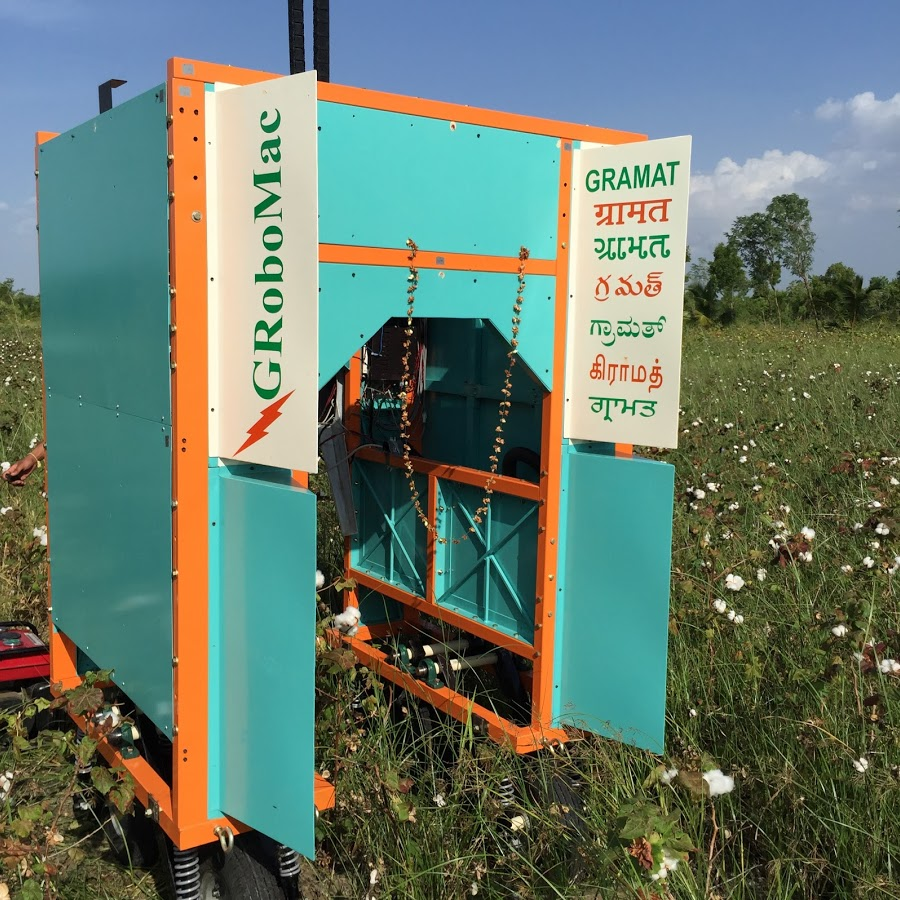
\includegraphics[width=.9\linewidth]{./images/grobomac.png}
\caption{Grobomac Cotton Machine}
\end{figure}
\end{column}
\end{columns}
\end{frame}

\begin{frame}[label={sec:org0abf73e}]{The Internet of Things in farming}
\begin{columns}
\begin{column}{0.5\columnwidth}
\begin{itemize}
\item IoT and wireless sensor node can
reduce time and efforts required for
monitoring the agriculture
environment.
\item Different organizations, government
departments etc., are taking
interest in implementing the
technology for agriculture
parameters measurement.
\end{itemize}
\end{column}
\begin{column}{0.5\columnwidth}
\begin{figure}[htbp]
\centering
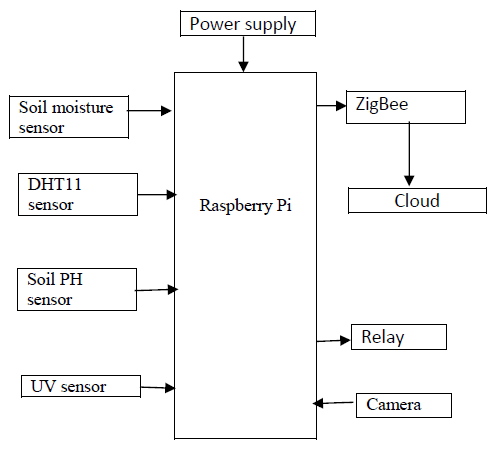
\includegraphics[width=.9\linewidth]{./images/config.png}
\caption{Raspberry Pie Example Configuration}
\end{figure}
\end{column}
\end{columns}
\end{frame}
\begin{frame}[label={sec:orgeaad533}]{Data: Acquisition}
\begin{figure}[htbp]
\centering
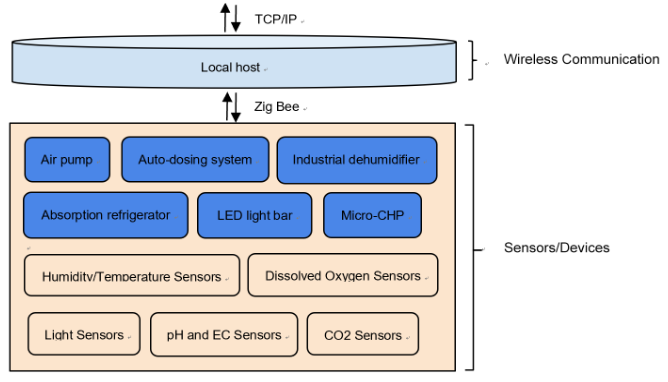
\includegraphics[width=.9\linewidth]{./images/dataaq.png}
\caption{Data Acquisition Architecture}
\end{figure}
\end{frame}
\begin{frame}[label={sec:org178d062}]{Data: Processing}
\begin{figure}[htbp]
\centering
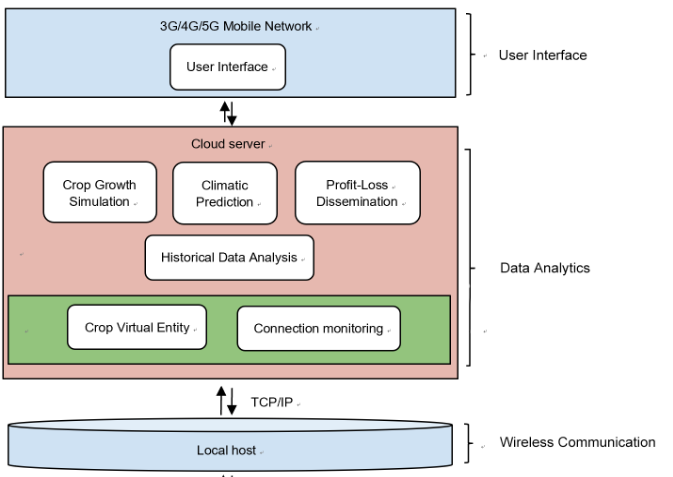
\includegraphics[height=60mm]{./images/datapro.png}
\caption{Data Processing using Virtual Machines}
\end{figure}
\end{frame}
\begin{frame}[label={sec:org3768414}]{Way Forward: An integrated system}
\begin{itemize}
\item IoT's monitoring systems, Data processing and analytics using a centralized server and finally ground work using robotics is the future.
\item Challenges faced:
\begin{itemize}
\item Scale of the project
\item Initial development and prototyping cost
\item Lack of Open Research and Data.
\end{itemize}
\item If implemented the farming will be a much more viable career
choice for a lot of people.
\item Losses due to unpredictable climatic conditions which forces a
large number of farmers to suicide can be avoided.
\end{itemize}
\end{frame}
\begin{frame}[label={sec:orgd3f561c}]{Conclusion}
\begin{itemize}
\item An integrated system that leverages IoT, Open Data and Robotics is
going to be future of agriculture.
\item Even though the technology in itself has reached enough maturity,
adoption rates of similar systems in mainstream agriculture by independent
farmers is rare.
\item Startups are venturing into agri-tech is increasing constantly.
\end{itemize}
\end{frame}
\begin{frame}[label={sec:org0908aa9}]{References}
\begin{itemize}
\item Li,  N.P.,  Xiao,  Y.M.,  Shen,  L.,  Xu,  Z.Y.,  Li,  B.T.  and  Yin,  C.X.
(2019) \emph{Smart   Agriculture   with   an   Automated  IoT-Based  Greenhouse
System  for  Local  Communities. Advances  in  In-ternet of Things} ,
9, 15-31. \url{https://doi.org/10.4236/ait.2019.92002}
\item Sudhir Rao Rupanagudi, Ranjani B. S., Prathik Nagaraj, Varsha G Bhat,
and Thippeswamy G, \emph{A Noveli Cloud Computing based Smart Farming System
for Early Detection of Borer Insects in Tomatoes} , ICCICT, pp.1-6, 2015.
\item Duan Yan-e, \emph{Design of Intelligent Agriculture Management Information
System Based on IoT}, Fourth International Conference on Intelligent
Computation Technology and Automation, Volume-1, pp. 1045-1049, 2011
\end{itemize}
\end{frame}
\end{document}
